\chapter{Strömungssimulation mit der Lattice-Boltzmann-Methode}
\section{Kinetische Theorie und Boltzmann-Gleichung}
\begin{itemize}
\item $N$ Teilchen (Atome, Moleküle, ...) mit den Größen
\item  $\vec{x}_i \in \real^3$ ... Position des $i$-ten Teilchens,
\item $\vec{p}_i \in \real^3$ ... Impuls des $i$-ten Teilchens.
\end{itemize}

Mikroskopische Bewegungsgleichungen
\begin{equation}
 \diff{\vec{x}_i}{t} = \pdiff{H}{\vec{p_i}}, \qquad \diff{\vec{p}_i}{t} = -
  \pdiff{H}{\vec{x}_i}.
\end{equation}
Dabei ist $H$ die \emph{Hamilton-Funktion} (Gesamtenergie) des Systems in
Abhängigkeit aller Positionen $(\vec{x}_1, \ldots, \vec{x}_N)$ und Impulse $(\vec{p}_1, \ldots,
\vec{p}_N)$ und
\[ \pdiff{H}{\vec{p}_i} = \left( 
    \pdiff{H}{p_{i,1}}, \pdiff{H}{p_{i,2}}, \pdiff{H}{p_{i,3}}
   \right)^\top. \]
Typische Form von $H$:
\begin{equation}
  H = \sum_{i=1}^N \left( \frac{|\vec{p}_i|^2}{2m} + U(\vec{x}_i) \right)
  + \rez{2} \sum_{\substack{i,j=1\\i \ne j}}^N V(\vec{x}_i - \vec{x}_j),
\end{equation}
wobei
\begin{itemize}
\item $\frac{|\vec{p}_i|^2}{2m}$ ... Kinetische Energie,
\item $U(\vec{x}_i)$ ... externes Potential, zum Beispiel Gravitationsfeld,
  elektrisches Feld,
\item $V(\vec{x}_i - \vec{x}_j)$ ... paarweises Interaktionspotenzial.
\end{itemize}

Mit 
\[ |\vec{p}_i|^2 = p_{i,1}^2 + p_{i,2}^2 + p_{i,3}^2 \]
folgt dann
\begin{equation}
  \pdiff{H}{\vec{p_i}} = \left( 
    \pdiff{H}{p_{i,1}}, \pdiff{H}{p_{i,2}}, \pdiff{H}{p_{i,3}}
  \right)^\top  = \frac{\vec{p}_i}{m}.
\end{equation}
Damit gilt für die Geschwindigkeit $\vec{v} = \diff{\vec{x}_i}{t}$
\begin{equation}
  \diff{\vec{x}_i}{t} = \frac{\vec{p}_i}{m}.
\end{equation}

Wichtige Eigenschaft auf mikroskopischer Beschreibungsebene: Das System ist
invariant unter Zeitumkehr. Umkehr aller Impulse $\vec{p}_i \to - \vec{p}_i$ bei
$t=0$ führt zu
\[ \vec{x}_i'(t) = x_i(-t), \]
das System ``läuft rückwarts in der Zeit''.

\subsubsection*{Phasenraum}
Jeder Mikrozustand ist ein einzelner Punkt $(\vec{x}_1, \ldots, \vec{x}_N,
\vec{p}_1, \ldots, \vec{p}_N)$ im Phasenraum $\real^{6N}$. Zusammen mit den
Anfangs- und Randbedingungen ist die Zeitentwicklung des mikroskopischen Systems
eindeutig festgelegt. Aber:
\begin{itemize}
\item Die numerische Berechnung ist in der Praxis nicht durchführbar: Es gilt $N
  \gg 1$\footnote{%
    Loschmidt-Konstante \SI{2.6e25}{\per \m \cubed}, Anzahl der Moleküle pro
    Kubikmeter eines idealen Gases unter Normalbedingungen}
  und man kann die Anfangsorte und -geschwindigkeiten aller einzelnen Teilchen
  nicht messen.
\item ``Interessante'' Observablen wie Druck, Temperatur, usw. basieren auf
  Mittelung über viele mikroskopische Trajektorien.
\end{itemize}
$\rightsquigarrow$ Statistische Beschreibung.

Idee: Beschreibe Gas oder Flüssigkeit durch eine Wahrscheinlichkeitsdichte
$f(\vec{x}, \vec{p}, t)$: ``Wahrscheinlichkeit, ein Teilchen am Ort $\vec{x}$
mit Impuls $\vec{p}$ zum Zeitpunkt $t$ zu finden''.
\[ \int_R f(\vec{x}, \vec{p}, t) \diffop^3 \times \diffop^3 p =
  \frac{\text{Anzahl Teilchen im Raum $R$}}{\text{Gesamtzahl der Teilchen}} \]
Ludwig Boltzmann 1872: Herleitung der zeitlichen Evolution von $f(\vec{x},
\vec{p}, t)$ ausgehend von der mikroskopischen Beschreibung.

\subsubsection*{Boltzmann-Gleichung}
\[ \partial_t f + \frac{\vec{p}}{m} \cdot \partial_{\vec{x}} f + \vec{F} \cdot
  \partial_{\vec{p}} f = C[f] \]
$m$ ... Masse eines Teilchens, \\
$C[f]$ ... Kollisionsoperator.
\[ \frac{\vec{p}}{m} \cdot \partial_{\vec{x}} f =
  \frac{p_1}{m} \cdot \partial_{x_1} f +
  \frac{p_2}{m} \cdot \partial_{x_2} f +
  \frac{p_3}{m} \cdot \partial_{x_3} f \]
Analog
\[ \vec{F} \cdot \partial_{\vec{p}} f = \sum_{i=1}^3 F_i \cdot \partial_{p_i}
  f. \]

Linke Seite der Gleichung: Gleichförmige Flussbewegung
\[ \partial_t f + \frac{\vec{p}}{m} \cdot \partial_{\vec{x}} f + \vec{F} \cdot
  \partial_{\vec{p}} f = 0 \tag{$\circ$} \]
wird gelöst von
\[ f( \vec{x}, \vec{p}, t ) = g \left( \vec{x} - \frac{\vec{p}}{m} \cdot t,
    \vec{p} - \vec{F} \cdot t \right) \]
für eine beliebige (differenzierbare) Funktion $g( \vec{x}, \vec{p} )$.
Einsetzen in ($\circ$)
\[ \underbrace{(\partial_{\vec{x}} g) \cdot \left( - \frac{\vec{p}}{m} \right) +
  (\partial_{\vec{p}} g) \cdot (-\vec{F})}_{\partial_t f} +
  \frac{\vec{p}}{m} \cdot \partial_{\vec{x}} g +
  \vec{F} \cdot \partial_{\vec{p}} g = 0
\]

Allgemein: Interpretation der linken Seite als ``totale Zeitableitung''
\[ \diff{}{t} f( \vec{x}(t), \vec{p}(t), t ) =
  \partial_{\vec{x}} f \cdot \underbrace{\diff{\vec{x}(t)}{t}}_{\vec{p}/m} +
  \partial_{\vec{p}} f \cdot \underbrace{\diff{\vec{p}(t)}{t}}_{\vec{F}} +
  \partial_t f.
\]

\subsubsection*{Kollisionsoperator $C[f]$}
Exakte Herleitung benötigt die Zwei-Teilchen Wahrscheinlichkeitsdichte
\[ f^{(2)}( \vec{x}_1, \vec{p}_1, \vec{x}_2, \vec{p}_2), \]
sie beschreibt die Wahrscheinlichkeit, ein Teilchen mit $(\vec{x}_1, \vec{p}_1)$
und ein Teilchen mit $(\vec{x}_2, \vec{p}_2)$ zu finden.

Zur Bestimmung von $f^{(2)}$ benötigen wir $f^{(3)}$, für die Bestimmung von
$f^{(3)}$ brauchen wir $f^{(4)}$, ... für $f^{(N-1)}$ brauchen wir $f^{(N)}$.
Systeme mit einer großen Anzahl von Teilchen nennt man
BBGKY\footnote{Bogoliubov, Born, Green, Kirkwood, Yvon}-Hierarchien
$\rightsquigarrow$ Eine exakte Lösung der ursprünglichen $N$-Teilchen Problems ist
nicht durchführbar.

Ausweg: Approximationen, um Kollisionsoperator allein durch $f$ auszudrücken.

Dazu treffen wir einige Annahmen:
\begin{enumerate}
\item ``Verdünntes'' Gas mit kurzreichweitiger Wechselwirkung, Teilchen
  befinden sich die meiste Zeit im freien Flug, nur gelegentlich kollidieren zwei
  Teilchen \emph{elastisch}\footnote{%
    Es gelten Impuls- und Energieerhaltung. Insbesondere wird keine Energie in
    Form von Wärme oder Verformung verloren.
  } und ändern ihre Flugbahnen.
  \[ \vec{p} + \vec{p}_* = \vec{p}\,' + \vec{p}_*\,', \qquad
    \frac{|\vec{p}|^2}{2m} + \frac{|\vec{p}_*|^2}{2m} =
    \frac{|\vec{p}\,'|^2}{2m} + \frac{|\vec{p}_*\,'|^2}{2m}. \]
\item Molekulares Chaos bzw. ``Stoffzahlansatz'' (Boltzmann 1872), $f^{(2)}$
  faktorisiert unmittelbar vor der Kollision, das heißt
  \[ f^{(2)}( \vec{x}_1, \vec{p}_1, \vec{x}_2, \vec{p}_2, t) \approx
    f(( \vec{x}_1, \vec{p}_1, t) \cdot f(\vec{x}_2, \vec{p}_2, t ). \]
  Also sind die Wahrscheinlichkeitsverteilungen der Teilchen unkorreliert.

  \emph{Aber:} Diese Annahme gilt nicht mehr unmittelbar nach der Kollision.
  Somit wird implizit eine Zeitrichtung festgelegt und das System wird
  irreversibel.
\end{enumerate}

Kollisionsoperator $C[f]$:
\begin{align*}
  &C[f] ({\color{blue} \vec{x}}, {\color{red} \vec{p}}, t) = \\
  &\int_{\real^3} \int_{\sphere^2}
  B(\vec{p} - \vec{p}_*, \vec{n})
  \big(
  f( {\color{blue}\vec{x}}, \vec{p}\,', t ) \cdot
  f( {\color{blue}\vec{x}}, \vec{p}_*\,', t ) -
  f( {\color{blue}\vec{x}}, {\color{red} \vec{p}}, t ) \cdot
  f( {\color{blue}\vec{x}}, \vec{p}_*, t )
  \big)
  \diffop^2 n \diffop^3 p_*.
\end{align*}
$\vec{p}\,'$ und $\vec{p}_*\,'$ im Integranden sind Funktionen von $\vec{p}$ und
$\vec{p}_*$, festgelegt durch Impuls- und Energieerhaltung.
\[ \begin{aligned}
    \vec{p}'
    &= \vec{p} - ( \vec{n} \cdot ( \vec{p} - \vec{p}_* ) ) \cdot \vec{n} \\
    \vec{p}_*\,'
    &= \vec{p}_* - ( \vec{n} \cdot ( \vec{p}_* - \vec{p} ) ) \cdot \vec{n}
  \end{aligned}
\]
$B( \vec{p} - \vec{p}_*, \vec{n} )$ ist der \emph{Streuquerschnitt}, er bildet
mikroskopische Details der Kollision ab. Beispiel: ``Harte Kugeln''
\[ B( \vec{p} - \vec{p}_*, \vec{n} ) = \begin{cases}
    \vec{n} \cdot ( \vec{p} - \vec{p}_* ), &
    \vec{n} \cdot ( \vec{p} - \vec{p}_* ) \ge 0, \\
    0, & \text{sonst.}
  \end{cases}
\]
Anmerkung: $B$ hängt im Allgemeinen nur von $|\vec{p}-\vec{p}_*|$ und $\vec{n}
\cdot \frac{\vec{p}-\vec{p}_*}{|\vec{p}-\vec{p}_*|}$ ab.

\subsubsection*{Interpretation der $f$-Terme im Integranden von $C[f]$}
\[ f( \vec{x}, \vec{p}\,', t ) \cdot f( \vec{x}, \vec{p}_*\,', t ) \]
lässt sich als ``gain term'' auffassen. Nach der Kollision gibt es ein
zusätzliches Teilchen mit Impuls $\vec{p}$, das heißt $f( \vec{x}, \vec{p}, t )$
in der Boltzmann-Gleichung nimmt zu.
\[ - f( \vec{x}, \vec{p}, t ) \cdot f( \vec{x}, \vec{p}_*, t ) \]
lässt sich als ``loss term'' auffassen. Aufgrund der Kollision ``verschwindet''
ein Teilchen mit Impuls $\vec{p}$, das heißt $f( \vec{x}, \vec{p}, t )$ nimmt
ab.

\section{Kollisionsinvarianten und Erhaltungssätze}
Beispiel: Gesamte kinetische Energie des Systems:
\[ E(t) = \int_{\real^3} \int_{\real^3} \frac{|\vec{p}|}{2m} f( \vec{x},
  \vec{p}, t ) \diffop^3 p \diffop^3 x. \]
Der Einfachheit halber nehmen wir an, dass $f$ räumlich homogen ist, also nicht
von $x$ abhängt. Außerdem sollen keinen externen Kräfte existieren, somit
vereinfacht sich die Boltzmann-Gleichung zu
\[ \partial_t f = C[f]. \tag{$\circ$} \]
Zeitliche Änderung der Gesamtenergie:
\[ \diff{}{t} E(t) 
  = \int_{\real^3} \frac{|\vec{p}|}{2m} \partial_t f( \vec{p}, t ) \diffop^3 p
  \overset{(\circ)}{=} \int_{\real^3} \frac{|\vec{p}|}{2m} C[f] \diffop^3 p. \]
Somit folgt, dass die Energieerhaltung $\diff{}{t} E(t) = 0$ äquivalent ist zu
\[ \int_{\real^3} \frac{|\vec{p}|}{2m} C[f] \diffop^3 p = 0. \]

\emph{Verallgemeinerung:} Für welche Funktionen $\varphi(\vec{p})$ gilt
\[ \int_{\real^3} \varphi(\vec{p}) C[f] \diffop^3 p = 0 \, ? \]
Wir setzen $C[f]$ ein und verwenden die Abkürzungen
\[ f( \vec{x}, \vec{p}\,', t ) =: f', \qquad
  f( \vec{x}, \vec{p}_*\,', t ) =: f_*', \qquad
  f( \vec{x}, \vec{p}, t ) =: f, \qquad
  f( \vec{x}, \vec{p}_*, t ) =: f_*. \]
Damit 
\begin{align*}
  \int_{\real^3} \varphi(\vec{p}) C[f] \diffop^3 p
  &= \int_{\real^3} \int_{\real^3} \int_{\sphere^2}
    \varphi(\vec{p})
    B(\vec{p} - \vec{p}_*, \vec{n}) \cdot
    \big( f' f_*' - f f_* \big)
    \diffop^2 n \, \diffop^3 p_* \, \diffop^3 p \\
  \intertext{Substitution: $\vec{p} \leftrightarrow \vec{p}_*$,
  $\vec{p}\,' \leftrightarrow \vec{p}_*\,'$, $\vec{n} \leftrightarrow -\vec{n}$}
  &= \int_{\real^3} \int_{\real^3} \int_{\sphere^2}
    \varphi( \vec{p}_* )
    \underbrace{B(\vec{p}_* - \vec{p}, - \vec{n})}_{= B(\vec{p} - \vec{p}_*, \vec{n})} \cdot
    \underbrace{(f_*' f' - f_* f)}_{=f' f_*' - f f_*}
    \diffop^2 n \, \diffop^3 p_* \, \diffop^3 p.
\end{align*}
Mit der Abkürzung $B(\vec{p}_* - \vec{p}, - \vec{n}) =: B$ folgt also:
\[ \iiint \varphi(\vec{p}) \cdot B \cdot (f' f_*' - f f_*)
  \diffop^2 n \, \diffop^3 p_* \, \diffop^3 p
  = \iiint \varphi(\vec{p}_*) \cdot B \cdot (f' f_*' - f f_*)
  \diffop^2 n \, \diffop^3 p_* \, \diffop^3 p. \]
Wir können das Integral auch bezüglich $(\vec{p}\,'$, $\vec{p}_*\,')$ anstelle
von ($\vec{p}$,$\vec{p}_*$) ausdrücken, unter der Annahme, dass die Determinante
der Jacobi-Matrix $=1$ ist:
\begin{align*}
  \iiint \varphi(\vec{p}) \cdot B \cdot (f' f_*' - f f_*)
    \diffop^2 n \, \diffop^3 p_* \, \diffop^3 p
  &= \iiint \varphi(\vec{p}) B (f' f_*' - f f_*)
    \diffop^2 n \, \diffop^3 p_*{\color{red}'} \, \diffop^3 p{\color{red}'} \\
  \intertext{Umbenennung: $(\vec{p}, \vec{p}_*) \leftrightarrow (\vec{p}\,',
  \vec{p}_*\,')$}
  &= \iiint \varphi(\vec{p}\,') \cdot B \cdot
    \underbrace{(f f_* - f' f_*')}_{= - (f'f_*' - ff_*)}
    \diffop^2 n \, \diffop^3 p_* \, \diffop^3 p
\end{align*}
Wie zuvor kann man kann wieder $\vec{p} \leftrightarrow \vec{p}_*$
substituieren.

Insgesamt erhalten wir
\begin{align*}
  \int_{\real^3} \varphi(\vec{p}) C[f] \diffop^3 p
  &= \iiint \varphi(\vec{p}) \cdot B \cdot (f' f_*' - f f_*)
    \diffop^2 n \, \diffop^3 p_* \, \diffop^3 p \\
  &= \iiint \varphi(\vec{p}_*) \cdot B \cdot (f' f_*' - f f_*)
    \diffop^2 n \, \diffop^3 p_* \, \diffop^3 p \\
  &= - \iiint \varphi(\vec{p}\,') \cdot B \cdot (f' f_*' - f f_*)
    \diffop^2 n \, \diffop^3 p_* \, \diffop^3 p \\
  &= - \iiint \varphi(\vec{p}_*\,') \cdot B \cdot (f' f_*' - f f_*)
    \diffop^2 n \, \diffop^3 p_* \, \diffop^3 p.
\end{align*}
Addiere alle vier Varianten zusammen:
\[ \begin{aligned}
    \int_{\real^3} \varphi(\vec{p}) \cdot C[f] \diffop^3 p =
    \iiint \rez{4} &\big( \varphi(\vec{p}) + \varphi(\vec{p}\,') - \varphi( \vec{p}\,')
    - \varphi( \vec{p}_*\,') \big) \\
    &\cdot B( \vec{p} - \vec{p}_*, \vec{n} )
    \cdot (f'f_*' - ff_*) \,
    \diffop^2 n \, \diffop^3 p_* \, \diffop^3 p.
  \end{aligned}
\]
Somit erhalten wir 0 und damit auch die Energieerhaltung, wenn 
\[ \varphi( \vec{p} ) + \varphi( \vec{p}_* ) = \varphi( \vec{p}\,' ) + \varphi(
  \vec{p}_*') \]
für alle $\vec{p}, \vec{p}_* \in \real^3$ ($\vec{p}\,', \vec{p}_*'$ sind
Funktionen von $\vec{p}, \vec{p}_*$). Funktionen $\varphi$ mit dieser Eigenschaft heißen \emph{Kollisionsinvarianten}.

Es stellt sich heraus: Die Allgemeine Lösung
\[ \varphi( \vec{p} ) = a + \vec{b} \cdot \vec{p} + \rez{2} c |\vec{p}|^2 \]
ist Kollisionsinvariante für beliebige Konstanten $a \in \real$, $\vec{b} \in
\real^3$, $c \in \real$.

Daraus folgt zum Beispiel für die Impulserhaltung $\vec{p} + \vec{p}_* =
\vec{p}\,' + \vec{p}_*\,'$ $\Rightarrow$
\[ \vec{b} \cdot \vec{p} + \vec{b} \cdot \vec{p}_*
  = \vec{b} \cdot \vec{p}\,' + \vec{b} \cdot \vec{p}_*\,'. \]
Analog für die Energieerhaltung.

Verschiedene Werte für $a,b,c$ liefern die bekannten Erhaltungssätze. Für
$\varphi(\vec{p}) = 1$ folgt die Dichteerhaltung
\[ \int_{\real^3} C[f] \diffop^3 p = 0. \]
Für $\varphi(\vec{p}) = \vec{p}$ folgt die Impulserhaltung
\[ \int_{\real^3} \vec{p} \cdot C[f] \diffop^3 p = 0. \]
Für $\varphi(\vec{p}) = \rez{2m} |p|^2$ folgt die Energieerhaltung
\[ \int_{\real^3} \frac{|p|^2}{2m} C[f] \diffop^3 p = 0. \]

\section{Thermisches Gleichgewicht und H-Theorem}
Im Folgenden betrachte räumlich homogene Verteilungen\footnote{%
  Das heißt $f$ hängt nicht von $\vec{x}$ ab.}
und keine externen Kräfte. Somit vereinfacht sich die linke Seite der
Boltzmann-Gleichung zu $\partial_t f( \vec{p}, t)$:
\[ \partial_t f = C[f]. \tag{B'} \]
Was sind die Gleichgewichtslösungen der Boltzmann-Gleichung als Funktionen $f$
mit $C[f] = 0$ (also $C[f]$ ist die Nullfunktion)?

Zentrale Größe zum ``Messen'' der Annäherung ans Gleichgewicht ist die
\emph{Entropie} (``Unordnung''):
\[ S(t) := - \int_{\real^3} f( \vec{p}, t ) \log( f( \vec{p}, t) \diffop^3 p. \]
Sie wird mit $S$ bezeichnet. Es wird auch die Bezeichnung $-S = H$ verwendet.

Wir leiten nach der Zeit ab und setzen die Boltzmann-Gleichung (B') ein:
\[ \begin{aligned}
    \diff{}{t} S(t) &= - \int (\partial_t f) \log f + f \rez{f} \partial_t f
    \diffop^3 p. \\
    &\overset{(\text{B'})}{=}
    - \int \log f C[f] \diffop^3 p + \int 1 \cdot C[f] \diffop^3 p
  \end{aligned}
\]
Es gilt $\int 1 \cdot C[f] \diffop^3 p = 0$ wegen der Dichteerhaltung.

\begin{thm}[Boltzmann's H-Theorem]
  Die Entropie nimmt monoton zu ($\diff{}{t} S(t) \ge 0$), das heißt
  \[ - \int_{\real^3} \log f \cdot C[f] \diffop^3 p \ge 0 \]
  für positive Funktionen $f$ ($f(\vec{p}, t) > 0$).

  Gleichheit gilt genau dann, wenn
  \[ f(\vec{p}) = \exp \left( a + \vec{b} \cdot \vec{p} + \rez{2} c |\vec{p}|^2
      \right) \tag{$\ast$} \] 
  für Konstanten $a, \vec{b}, c < 0$.
\end{thm}

\begin{rmrk*}
  Wenn $f$ von der oben genannten Form ist, dann strebt $S(t)$ asymptotisch
  gegen einen Gleichgewichtswert (siehe C. Villani).
\end{rmrk*}

Die Gleichgewichtslösungen sind also genau von der Form ($\ast$).

``$\Rightarrow$'' Sei $f$ Gleichgewichtslösung, also $C[f] \equiv 0$. Dann gilt
\[ \int \log f C[f] \diffop^3 p = \int \log f \cdot 0 \diffop^3 p = 0. \]
Aus der Äquivalenz im H-Theorem folgt dann, dass $f$ die Form ($\ast$) hat.

``$\Leftarrow$'' Setze $\varphi(\vec{p}) = \log f = a + b \cdot \vec{p} +
\rez{2} c |p|^2$. $\varphi$ ist Kollisionsinvariante, also
\[ \begin{aligned}
    \varphi(\vec{p}) + \varphi(\vec{p}_*) &= \varphi(\vec{p}\,') +
    \varphi(\vec{p}_*\,' \\
    \log f + \log f_* &= \log f' + \log f_*' \\
    \log( f \cdot f_* ) &= \log( f' \cdot f_*' ) \\
    f \cdot f_* &= f' \cdot f_*'.
  \end{aligned}
\]
Einsetzen in $C[f]$ ergibt $C[f] \equiv 0$.

\begin{proof}[Beweis des H-Theorems]
Es gilt (siehe ...)
\[ \begin{aligned}
    \int_{\real^3} \varphi(\vec{p}) \cdot C[f] \diffop^3 p =
    \iiint \rez{4}
    &\big( \varphi(\vec{p}) + \varphi(\vec{p}\,') - \varphi(\vec{p}\,') 
    - \varphi( \vec{p}_*\,') \big) \\
    &\cdot B( \vec{p} - \vec{p}_*, \vec{n} )
    \cdot (f'f_*' - ff_*) \,
    \diffop^2 n \, \diffop^3 p_* \, \diffop^3 p.
  \end{aligned}
\]
Setze $\varphi(\vec{p}) = \log f(\vec{p}, t)$ ($f$ festgehalten):
\[ \begin{aligned}
    \int_{\real^3} \log f \cdot C[f] \diffop^3 p &=
    - \rez{4} \iiint
    \underbrace{\big( \log f + \log f_*
      - \log f' - \log f_*' \big)}_{\log \frac{f f_*}{f' f_*'}}
    (f' f_*' - f f_* ) \cdots \\
    &= -\rez{4} \iiint f' f_*' (1 - \lambda) \log \lambda \cdot B( \vec{p} -
    \vec{p}_*, \vec{n} ) \,
    \diffop^2 n \, \diffop^3 p_* \, \diffop^3 p.
  \end{aligned}
\]
mit $\lambda( \vec{p}, \vec{p}_*) := \frac{f f_*}{f' f_*'} > 0$, da $f > 0$ laut
Annahme.

Es gilt $B( \vec{p} - \vec{p}_*, \vec{n} ) \ge 0$ (der Streuquerschnitt ist
nicht-negativ) und
\[ - (1-\lambda) \log \lambda \ge 0 \]
für alle $\lambda > 0$ wobei Gleichheit genau dann gilt, wenn $\lambda = 1$.

Somit folgt
\[ -\rez{4} \iiint f' f_*' (1 - \lambda) \log \lambda \cdot B( \vec{p} -
  \vec{p}_*, \vec{n} ) \,
  \diffop^2 n \, \diffop^3 p_* \, \diffop^3 p \ge 0, \]
also $\diff{}{t} S(t) \ge 0$.

Was folgt aus $- \int \log f C[f] \diffop^3 p = 0$? Dann muss der Integrand
überall $=0$ sein, da $\log f$ und $C[f]$ stets $\ge 0$ sind. Es muss also $B(
\vec{p} -  \vec{p}_*, \vec{n} ) = 0$ sein oder $\lambda( \vec{p}, \vec{p}_*) =
1$ für alle $\vec{p}, \vec{p}_* \in \real^3$.

Bis auf Spezialfälle gibt es immer ein $\vec{n} \in \sphere^2$ mit $B(
\vec{p} -  \vec{p}_*, \vec{n} ) > 0$, also muss $\lambda( \vec{p}, \vec{p}_*) =
1$ gelten.
\[ \lambda( \vec{p}, \vec{p}_* ) = 1 \qLRq f f_* = f' f_*' \qLRq \log f + \log
  f_* = \log f' + \log f_*', \]
also ist $\varphi(\vec{p}) = \log f(\vec{p}, t)$ eine Kollisionsinvariante.
Damit existieren $a \in \real$, $b \in \real^3$ und $c \in \real$, sodass
\[ \varphi( \vec{p} ) = a + \vec{b} \cdot \vec{p} + \rez{2} c |\vec{p}|^2, \]
also gilt
\[ f( \vec{p}, t ) = \exp \left( a + \vec{b} \cdot \vec{p} + \rez{2} c
    |\vec{p}|^2 \right) \]
($c < 0$ wegen Integrierbarkeit).
\end{proof}

\begin{rmrk*}
  Man kann die Gleichgewichtslösungen $\exp \left( a + \vec{b} \cdot \vec{p} +
    \rez{2} c |\vec{p}|^2 \right)$ umschreiben als
  \[ f_{\mathrm{MB}}(\vec{p}) = \rho \left( \frac{\beta}{2 \pi m}
    \right)^{\frac{3}{2}} \exp \left( - \beta \rez{2m} |\vec{p}- m\vec{u}|^2
    \right) \]
  mit Dichte $\rho$ und $\beta = \rez{k_B T}$. Diese Form bezeichnet man als
  \emph{Maxwell-Boltzmann-Verteilung}. Das ist eine Gauß-Funktion.

  Der Normalisierungsfaktor $\left( \frac{\beta}{2 \pi m} \right)^{\frac{3}{2}}$
  wird benötigt, um
  \[ \int_{\real^3} f_{\mathrm{MB}}(\vec{p}) \diffop^3 p = \rho \]
  sicherzustellen.

  Erhaltungssätze (Dichte-, Impuls- und Energieerhaltung) legen die Parameter
  $\rho$, $\vec{u}$ und $\beta$ der MB-Verteilung eindeutig fest. Das heißt, man
  kann allein aufgrund der erhaltenen Größen auf die asymptotische
  Gleichgewichtsverteilung schließen, $f(\vec{p}, t) \xrightarrow{n \to \infty}
  f_{\mathrm{MB}}(\vec{p})$.
  \[ \begin{aligned}
      \rho &= \int_{\real^3} f( \vec{p}, t ) \diffop^3 p, 
      \qquad \text{$\rho$ hängt nicht von $t$ ab.} \\
      \vec{u} &= \frac{\int_{\real^3} \frac{\vec{p}}{m} f(\vec{p}, t) \diffop^3
        p}{\int_{\real^3} f( \vec{p}, t ) \diffop^3 p}
      = \rez{\rho} \int_{\real^3} \frac{\vec{p}}{m} f(\vec{p}, t) \diffop^3 p \\
      E &= \frac{ \int_{\real^3} \frac{|\vec{p}|^2}{m}  f(\vec{p}, t) \diffop^3
        p}{\int_{\real^3} f(\vec{p}, t) \diffop^3 p}
    \end{aligned} \]
  Wähle $\beta$ so, dass $\frac{3}{2} \rez{\beta} + \rez{2} m |\vec{u}|^2 = E$.
  Dann erfüllt $f_{\mathrm{MB}}$ mit den Parametern $\rho$, $\vec{u}$, $\beta$
  \[ \begin{aligned}
      \int_{\real^3} f_{\mathrm{MB}}( \vec{p} ) \diffop^3 p &= \rho, \\
      \rez{\rho} \int \frac{\vec{p}}{m} f_{\mathrm{MB}}(\vec{p}) \diffop^3 p &=
      \vec{u}, \\
      \rez{\rho} \int \frac{|\vec{p}|^2}{m} f_{\mathrm{MB}}(\vec{p}) \diffop^3 p
      &= \frac{3}{2} \rez{\beta} + \rez{2} m |\vec{u}|^2 = E
    \end{aligned}
  \]
\end{rmrk*}

\section{Übergang zu makroskopischen Kontinuitätsgleichungen}
Ab jetzt soll wieder räumliche Abhängigkeit vorliegen, das heißt $f(\vec{x},
\vec{p}, t)$ hängt von $\vec{x}$. Somit gilt:
\begin{align*}
  \text{Dichte}& & \rho( \vec{x}, t)
  &= \int_{\real^3} f(\vec{x}, \vec{p}, t) \diffop^3 p \\
  \text{Geschwindigkeit}& & \vec{u}(\vec{x}, t)
  &= \rez{\rho(\vec{x}, t)} \int_{\real^3}
    \frac{\vec{p}}{m} f(\vec{x}, \vec{p}, t) \diffop^3 p \\
  \text{Gesamtenergie}& & E(\vec{x}, t)
  &= \rez{\rho(\vec{x}, t)} \int_{\real^3}
    \frac{|\vec{p}|^2}{2m} f(\vec{x}, \vec{p}, t) \diffop^3 p
\end{align*}
Relativgeschwindigkeit eines Teilchens:
\[ \vec{c} = \frac{\vec{p}}{m} - \vec{u}(\vec{x},t). \]
Es gilt
\[ \begin{aligned}
    \int_{\real^3} \vec{c} f(\vec{x}, \vec{p}, t) \diffop^3 p
    &= \int_{\real^3} \left(\frac{\vec{p}}{m} - \vec{u}(\vec{x},t) \right)
    f(\vec{x}, \vec{p}, t) \diffop^3 p \\
    &= \rho(\vec{x}, t) \vec{u}(\vec{x},t)
    - \vec{u}(\vec{x},t)
    \underbrace{\int_{\real^3} f \diffop^3 p}_{\rho} = 0
  \end{aligned}
  \tag{$\circ$}
\]
Somit gilt für $i,j \in \{1,2,3\}$:
\[ \left. \begin{aligned}
  \int_{\real^3} \frac{p_i}{m} \frac{p_j}{m} f \diffop^3 p
  &= \int (u_i + c_i)(u_j + c_j) f \diffop^3 p \\
  &= u_i u_j \underbrace{\int f \diffop^3 p}_{\rho}
    + u_i \underbrace{\int c_j f \diffop^3 p }_{= 0 (\circ)}
    + u_j \underbrace{\int c_i f \diffop^3 p }_{= 0 (\circ)}
    + \underbrace{\int c_i c_j f \diffop^3 p }_{=: \sigma_{ij}} \\
  &= \rho u_i u_j + \sigma_{ij}
\end{aligned} \quad \right\} \tag{$\ast$} \]
mit dem \emph(Spannungstensor) bzw. \emph{Drucktensor} (stress tensor)
$\sigma_{ij}$.

Die Gleichung gilt insbesondere auch für $j=i$. Also können wir mit
\[ |\vec{p}|^2 = \vec{p} \cdot \vec{p} = p_x p_x + p_y p_y + p_z p_z \]
die folgende Beziehung herleiten:
\begin{align*}
  \rho(\vec{x}, t) E(\vec{x}, t)
  &= \int_{\real^3} \frac{|\vec{p}|^2}{2m} f(\vec{x}, \vec{p}, t) \diffop^3 p \\
  &= \rho \rez{2} m |\vec{u}|^2 +
    \underbrace{\int \rez{2} m |\vec{c}|^2
    f \diffop^3 p}_{=\rez{2m}|\vec{p}-m \vec{u}|^2} \\
  &= \rho \rez{2} m |\vec{u}|^2 + \rho \rez{2} \eps( \vec{x}, t ),
\end{align*}
wobei $\eps$ die \emph{interne Energie} bezeichnet:
\[ \eps( \vec{x}, t ) := \rez{\rho(\vec{x},t)} \int \rez{2m} |\vec{p} - m
  \vec{u}(\vec{x},t)|^2 f(\vec{x}, \vec{p}, t) \diffop^3 p. \]

Für $i \in \{1, 2, 3\}$:
\begin{align*}
  \int \frac{p_i}{m} \frac{|\vec{p}|^2}{2m} f \diffop^3 p
  &= \int \rez{2} m (u_i + c_i) |\vec{u} + \vec{c}|^2 f \diffop^3 p \\
  &= \int \rez{2} m (u_i + c_i) ( |\vec{u}|^2
    + 2 \vec{u} \cdot \vec{c} + |\vec{c}|^2) f \diffop^3 p \\
  &= \rez{2} m u_i |\vec{u}|^2
    \underbrace{\int f \diffop^3 p}_{\rho}
    + m u_i \sum_{j=1}^3 u_j
    \underbrace{\int c_j f \diffop^3 p}_{= 0 (\circ)}
    + u_i \underbrace{\int \rez{2} m |\vec{c}|^2 f \diffop^3 p}_{\rho \eps} \\
  &\phantom{=} + \rez{2} m |\vec{u}|^2 \underbrace{\int c_i f \diffop^3 p}_{=0}
    + m \sum_{j=1}^3 u_j
    \underbrace{\int c_i c_j f \diffop^3 p}_{\sigma_{ij}}
    + \int c_i \rez{2} m |\vec{c}|^2 f \diffop^3 p \\
  &= \rho u_i \left( \rez{2} m |\vec{u}|^2 + \eps \right)
    + m \sum_{j=1}^3 u_j \sigma_{ij} + m q_i
\end{align*}
mit der \emph{Wärmestromdichte} (heat flux) $\vec{q}$:
\[ q_i = \int c_i \rez{2} |\vec{c}|^2 f \diffop^3 p, \qquad i \in \{ 1, 2, 3
  \}. \]

Strategie: Nutze Erhaltungssätze des Kollisionsoperators $C[f]$ aus, um
makroskopische Erhaltungsgleichungen herzuleiten.

Boltzmann-Gleichung:
\[ \partial_t f + \frac{\vec{p}}{m} \cdot \partial_{\vec{x}} f
  + \vec{F} \cdot \partial_{\vec{p}} f = C[f]. \]
Wir nehmen an, dass die externe Kraft $\vec{F}$ nicht vom Impuls $\vec{p}$
abhängt.

Multipliziere die Boltzmann-Gleichung von links mit $1$, $\frac{\vec{p}}{m}$,
$\frac{|\vec{p}|^2}{2m}$ und integriere über den Impuls $\vec{p}$.
$\rightsquigarrow$ Rechte Seite verschwindet aufgrund der Erhaltungssätze für
$C[f]$.

Multiplikation mit 1:
\begin{align*}
  \int \partial_t f \diffop^3 p
  + \int \frac{\vec{p}}{m} \cdot \partial_{\vec{x}} f \diffop^3 p
  + \int \vec{F} \cdot \partial_{\vec{p}} f \diffop^3 p
  &= 0 \\
  \partial_t \underbrace{\int f \diffop^3 p}_{\rho}
  + \sum_{j=1}^3 \partial_{x_j}
  \underbrace{\int \frac{p_j}{m} f \diffop^3 p}_{\rho u_j}
  + \sum_{j=1}^3 F_j
  \underbrace{\int \partial_{p_j} f \diffop^3 p}_{0}
  &= 0.
\end{align*}
Es gilt $\int \partial_{p_j} f \diffop^3 p = 0$, weil
\[ \lim_{|\vec{p}| \to \infty} f(\vec{p}) = 0, \quad \text{analog zu } \int_{-
    \infty}^\infty \diff{}{x} h(x) = 0 \text{ für } \lim_{x \to \infty} h(x) =
  0, \, \lim_{x \to - \infty} h(x) = 0. \]
Also folgt die Kontinuitätsgleichung für die Dichte:
\[ \boxed{ \partial_t \rho( \vec{x}, t ) + \partial_{\vec{x}} (\rho(\vec{x},t)
    \vec{u}(\vec{x},t)) = 0 }\]
Integration über ein räumlich geschlossenes Volumen $V$:
\[ \underbrace{\partial_t \int_V \rho(\vec{x},t) \diffop^3 x}_{A} +
  \underbrace{\int_V \partial_{\vec{x}} (\rho(\vec{x},t) \vec{u}(\vec{x},t))
    \diffop^3 x}_{B} = 0. \]
$A$ ist die zeitliche Änderung der Masse im Volumen. Für $B$ gilt nach dem
Integralsatz von Gauß:
\[ \int_V \partial_{\vec{x}} (\rho(\vec{x},t) \vec{u}(\vec{x},t))
  \diffop^3 x
  = \int_{\delta V} \rho(\vec{x},t) \vec{u}(\vec{x},t) \cdot \vec{n}(\vec{x})
  \diffop^3 p \]
mit dem Normalenvektor $\vec{n}$. Das lässt sich als die Masse, die durch den Rand
$\delta V$ hinein bzw. hinaus fließt, interpretieren.

Für Multiplikation mit $\frac{p_i}{m}$, $i \in \{1,2,3\}$:
\begin{align*}
  \partial_t
  \underbrace{\int \frac{p_i}{m} f \diffop^3 p}_{\rho u_i}
  + \sum_{j=1}^3 \partial_{x_j}
  \underbrace{\int \frac{p_i}{m} \frac{p_j}{m} f
  \diffop^3 p}_{\rho u_i u_j + \sigma_{ij}}
  + \sum_{j=1}^3 F_j
  \underbrace{\int \frac{p_i}{m} \partial_{p_j} f \diffop^3 p}_{C}
  = 0
\end{align*}
Für $C$ können wir partiell integrieren. Der zweite Term der partiellen
Integration verschwindet und es bleibt
\[ \int \frac{p_i}{m} \partial_{p_j} f \diffop^3 p = - \rez{m} \int
  \underbrace{(\partial_{p_j} p_i)}_{=\delta_{ij}} f \diffop^3 p
  = - \rez{m} \delta_{ij} \int f \diffop^3 p. \]
Damit gilt
\[ \sum_{j=1}^3 F_j \int \frac{p_i}{m} \partial_{p_j} f \diffop^3 p
  = - \rez{m} \rho F_i. \]

Also folgt die Kontinuitätsgleichung für den Impuls:
\[ \boxed{ \partial_t (\rho u_i) + \sum_{j=1}^3 \partial_{x_j} ( \rho u_i u_j +
    \sigma_{ij}) = \rez{m} \rho F_i }\]

Für Multiplikation mit $\frac{|\vec{p}|^2}{2m}$ folgt die Kontinuitätsgleichung
für die Energie
\[ \boxed{\partial_t \left( \rho \left( \rez{2} m |\vec{u}|^2 + \eps \right) \right)
+ \sum_{i=1}^3 \partial_{x_i} \left( \rho u_i \left( \rez{2} m |\vec{u}|^2 +
    \eps \right) + m \sum_{j=1}^3 u_j \sigma_{ij} + m q_i \right)
= \sum_{i=1}^3 \rho u_i F_i} \]

\subsubsection*{Rolle des Kollisionsoperators $C[f]$?}
``Schließen'' der Kontinuitätsgleichungen, das heißt Ausdrücken der Größen
$\sigma_{ij}$, $q_i$ durch $\rho$, $\vec{u}$, $\eps$ (``constitutive
equations'').

\subsubsection*{Umformung der Kontinuitätsgleichung für den Impuls}
\[ \partial_t (\rho u_i) +
  \sum_{j=1}^3 \partial_{x_j}( \rho u_i u_j + \sigma_{ij})
  = \rez{m} \rho F_i \]
für $i = 1,2,3$. Kettenregel anwenden:
\[ (\partial_t \rho) u_i + \rho \partial_t u_i + u_i \sum_{j=1}^3
  \partial_{x_j} (\rho u_j) + \sum_{j=1}^3 \rho u_j (\partial_{x_j} u_i) +
  \sum_{j=1}^3 \partial_{x_j} \sigma_{ij} = \rez{m} \rho F_i. \]
Aus der Kontinuitätsgleichung für die Dichte wissen wir, dass
\[ (\partial_t \rho) u_i + u_i \sum_{j=1}^3 \partial_{x_j} (\rho u_j) =  
  u_i \big( \partial_t \rho + \partial_{\vec{x}} \rho \vec{u} \big) = 0. \]
Also erhalten wir nach Multiplikation mit $\rez{\rho}$
\[ \partial_t u_i + \sum_{j=1}^3 u_j (\partial_{x_j} u_i) +
  \rez{\rho} \sum_{j=1}^3 \partial_{x_j} \sigma_{ij}
  = \rez{m} F_i. \]

Anmerkung: Eine analoge Schreibweise für $\sum_{j=1}^3 u_j (\partial_{x_j} u_i)$
ist
\[ (\vec{u} \cdot \nabla) u_i, \]
was sich als ``Ableitung in Richtung $\vec{u}$'' interpretieren lässt.

Analog zu oben setzen wir die Kontinuitätsgleichung für die Dichte und den
Impuls in die Kontinuitätsgleichung für die Energie ein und erhalten die
\emph{Kontinuitätsgleichung für die interne Energie}
\[ \boxed{ \rho \partial_t \eps
    + \sum_{j=1}^3 \left( \rho u_j \partial_{x_j} \eps
      + m \partial_{x_j} q_j \right)
    + m \sum_{i,j=1}^3 \sigma_{ij} \partial_{x_j} u_j
  = 0.} \]

\begin{rmrk*}
  \[ \rez{2} \int m \sum_{i=1}^3 c_i^2 \int \diffop^3 p =
    \rez{2} \int m |\vec{c}|^2 f \diffop^3 p =
    \rho \cdot \eps. \]
\end{rmrk*}

\section{Euler-Gleichungen der Strömungsmechanik}
\emph{Approximation:} Verteilungsfunktion $f(\vec{x},\vec{p},t)$ befindet sich
\emph{lokal} stets im (thermischen) MB-Gleichgewicht, das heißt
\[ f(\vec{x}, \vec{p}, t) = \rho(\vec{x},t)
  \left( \frac{\beta(\vec{x},t)}{2\pi m}\right)^{3/2} e^{-\beta(\vec{x},t)
    \rez{2m} |\vec{p} - m \vec{u}(\vec{x},t)|^2} \]
mit orts- und zeitabhängigen Parametern
\[ \rho(\vec{x}, t), \qquad \vec{u}(\vec{x}, t), \qquad \beta(\vec{x}, t). \]

Stelle Gleichung ($\ast$) nach $\sigma_{ij}$ um und nutze $c_i := \frac{p_i}{m}
- u_i$, es gilt $\diffop p = m \diffop c$.
\begin{align*}
  \sigma_{ij}
  &= \int c_i c_j f \diffop^3 p \\
  &= \int c_i c_j f m^3 \diffop^3 c \\
  &= \int c_i c_j \rho \left( \frac{\beta}{2\pi m}\right)^{3/2}
    e^{-\beta(\vec{x},t) \rez{2m} |\vec{p} - m \vec{u}(\vec{x},t)|^2}
    m^3 d^3 c \\
  &= \rez{m} \rho \rez{\beta} \partial_{ij}
\end{align*}
Für ideale Gase gilt  $\rez{m} \rho = \rez{m} \frac{Nm}{V} = \frac{N}{V}$. Aus Übungsaufgabe 7 wissen wir, dass $P = \frac{N}{\beta V}$. Also
\[ \sigma_{ij} =  P \cdot \delta_{ij}. \]
Zudem gilt
\[ \rez{2} m \sum_{i=1}^3 \sigma_{ii} = \rho \cdot \eps, \]
also
\[ \mathcal{P} = \rez{m} \frac{2}{3} \rho \cdot \eps. \]

Nun betrachten wir die Gleichung für $q_i$ und verwenden wieder $c_i = \frac{p_i}{m} - u_i$, also $\diffop p = m \diffop c$:
\begin{align*}
  q_i
  &= \int c_i \rez{2} |\vec{c}|^2 f \diffop^3 p \\
  &= \rho \left( \frac{\beta}{2\pi m}\right)^{3/2}
    \int c_i \rez{2} (c_x^2 + c_y^2 + c_z^2)
    e^{-\beta(\vec{x},t) \rez{2m} |\vec{p} - m \vec{u}(\vec{x},t)|^2}
    m^3 d^3 c.
\end{align*}
Der Integrand ist eine ungerade Funktion bezogen auf die Komponente $c_i$, also
folgt für $i = 1,2,3$:
\[ q_i = 0. \]

Setzen wir nun diese Ergebnisse in die Kontinuitätsgleichungen ein, erhalten
wir die \emph{Euler-Gleichungen der Strömungsmechanik} (im allgemeinen
kompressiblen Fall):
\[
  \boxed{ \quad
    \begin{aligned}
      \text{Dichte}& &
      \partial_ t \rho + \sum_{j=1}^3 \partial_{x_j} (\rho u_j) &= 0, \\
      \text{Impuls}& &
      \partial_t u_i + \sum_{j=1}^3 u_j \partial_{x_j} u_i + \rez{\rho}
      \partial_{x_j} P
      &= \rez{m} F_i \\
      \text{Interne Energie}& \quad & 
      \partial_t \eps + \sum_{j=1}^3 u_j \partial_{x_j} \eps +
      \frac{m}{\rho} P(\nabla \cdot \vec{u}) &= 0
    \end{aligned}
  \quad }
\]
Dabei ist
\[ \nabla \cdot \vec{u} = \sum_{j=1}^3 \partial_{x_j} u_j \]
die \emph{Divergenz} von $\vec{u}$.

\section{Navier-Stokes-Gleichungen}
\emph{Chapman-Enskog}: Störungstheorie der Boltzmann-Gleichung mit Knudsen-Zahl
$K_n$ als kleinem Parameter:
\[ K_n = \frac{\text{Mittlere freie Weglänge eines Moleküls}}
  {\text{Charakterisitsche makroskopische Länge}} \]
Zum Beispiel Durchmesser eines Rohrs, durch das die Strömung fließt.

Das führt zu den (viskosen, kompressiblen) Navier-Stokes-Gleichungen.

``constitutive equations''
\[ \sigma_{ij} = P \cdot \delta_{ij} - \tau_{ij} \]
\begin{itemize}
\item $P$ ... \emph{Druck},
\item $\tau_{ij}$ ... \emph{viskoser Spannungstensor}.
\end{itemize}
\begin{align*}
  \tau_{ij}
  &= \mu (\partial_{x_i} u_j + \partial_{x_j} u_i )
    + \lambda (\nabla \cdot \vec{u}) \delta_{ij} \\
  &= \underbrace{\left( \lambda + \frac{2}{3}\mu  \right)}_{\xi}
    (\nabla \cdot \vec{u}) \delta_{ij}
    + \mu ( \partial_{x_i} u_j + \partial_{x_j} u_i )
    - \frac{2}{3} \mu (\nabla \cdot \vec{u}) \delta_{ij}
\end{align*}
$\xi$ wird meist vernachlässigt, $\mu$ ist die \emph{dynamische Viskosität}.

\[ q_i = -\kappa \partial_{x_i} T \]
mit dem \emph{Wärmeleitkoeffizient} $\kappa$.

Für $i = 1,2,3$ gilt
\begin{align*}
  \sum_{j=1}^3 \partial_{x_j} \tau_{ij}
  &= \mu \sum_{j=1}^3 \left( \partial_{x_i} \partial_{x_j} u_j +
    \partial_{x_j}^2 u_i - \frac{2}{3} \delta_{ij} \partial_{x_j}
    (\nabla \cdot \vec{u}) \right) \\
  &= \mu \sum_{j=1}^3 \partial_{x_j}^2 u_i
    + \rez{3} \mu \partial_{x_i} (\nabla \cdot \vec{u}).
\end{align*}
Man benutzt den \emph{Laplace-Operator}
\[ \sum_{j=1}^3 \partial_{x_j}^2 =: \nabla^2 =: \Delta. \]

Setzen wir dies in die Kontinuitätsgleichung für den Impuls ein, erhalten wir
die \emph{kompressible Navier-Stokes-Impulsgleichung}. Für $i=1,2,3$ gilt
\[ \boxed{
    \rho \left(
      \partial_t u_i + \sum_{j=1}^3 u_j \partial_{x_j} u_i
    \right)
    \partial_{x_i} P
    = \mu \left(
      \nabla^2 \vec{u} + \rez{3} \partial_{x_i} (\nabla \cdot \vec{u})
    \right)
    + \rez{m} \rho F_i.
  } \]

Anmerkung: Im inkompressiblen Fall $\rho = \mathrm{const}$ verschwindet der
Term, $\rez{3} \partial_{x_i} (\nabla \cdot \vec{u})$, da
$\nabla \cdot \vec{u} = 0$.

\section*{Interpretation der Navier-Stokes-Gleichung}
\[ \sum_{j=1}^3 u_j \cdot \partial_{x_j} u_i \equiv (\vec{u} \cdot \nabla)
  u_i \]
beschreibt die \emph{Konvektion} des Geschwindigkeitsfelds von sich selbst.

Nicht-linearer Term in der Navier-Stokes-Gleichung.

Beispiel: Betrachte
\[ \partial_t h( \vec{x}, t ) + (\vec{u} \cdot \nabla) h(\vec{x},t) = 0 \]
mit $\vec{u} = \mathrm{const}$. Gesucht ist $h(\vec{x},t)$.

Lösung: Sei $h(\vec{x},t) = g(\vec{x} - t \vec{u})$ für eine beliebige
differenzierbare Funktion $g(\vec{x})$, dann sind 
\[ \partial_t h = \diff{}{t} g(\vec{x} - t \vec{u}) 
  = - \vec{u} \cdot \nabla g(\vec{x} - t \vec{u}) \]
und
\[ \nabla h = \nabla g. \]

Für Navier-Stokes ist $h = u_i$. Hier ist die Berechnung komplizierter, weil
$\vec{u}$ nicht konstant ist, sich selbst ``transportiert''.

Der Term
\[ \nabla^2 u_i \equiv \Delta u_i \equiv (\partial_x^2 + \partial_y^2 + 
  \partial_z^2) u_i \]
beschreibt die \emph{Diffusion} des Geschwindigkeitsfeldes.

Beispiel: Die Wärmeleitungsgleichung
\[ \partial_t ( \vec{x}, t ) - \mu \Delta h (\vec{x},t) = 0 \]
wird gelöst von
\[ h(\vec{x},t) = \rez{(\sqrt{4 \pi \mu t})^d}
  e^{-\frac{|\vec{x}|^2}{4 \mu t}} \]
mit der Dimension $d \in \{1,2,3\}$. Das ist eine Gauß-(Glocken-)Funktion, die
sich mit der Zeit verbreitert,
\[ \lim_{t \to 0} h(\vec{x},t) = \delta(\vec{x}), \]
wobei $\delta$ den Dirac-Impuls bezeichnet.

\section{Die Lattice-Boltzmann-Methode}
Grundlegende Idee: Diskretisiere die Verteilungsfunktion $f(\vec{x}, \vec{p}, t)$
der Boltzmann-Gleichung, um Navier-Stokes-Gleichung zu approximieren. Also wird
\begin{itemize}
\item $\vec{x}$ $\rightsquigarrow$ Reguläres kartesisches Gitter (diskrete,
  äquidistante Koordinaten),
\item $\vec{p}$ $\rightsquigarrow$ Geschwindigkeitsvektoren in Richtung der
  Nachbarfelder,
\item $t$ $\rightsquigarrow$ $t = 0, \Delta t, 2 \Delta t,
  \ldots$ Diskrete Zeitschritte.
\end{itemize}
Im zweidimensionalen Fall erhält man ein \emph{D2Q9-Schema} (zwei Dimensionen,
neun Geschwindigkeiten). Für drei Dimensionen ergibt sich ein
\emph{D3Q19-Schema}.
\begin{center}
  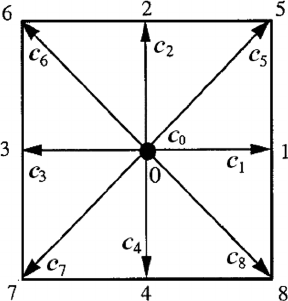
\includegraphics[width=5cm]{img/d2q9}
\end{center}
\begin{center}
  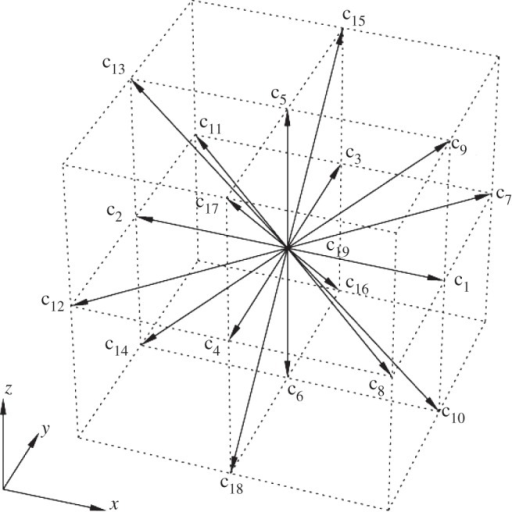
\includegraphics[width=10cm]{img/d3q19}
\end{center}

Diskrete Impulsvektoren für D2Q9:
\[ \vec{p}_i = \xi \cdot \vec{e}_i \]
mit
\begin{align*}
  \vec{e}_0 &= \pmat{0\\0},
            & \vec{e}_1 &= \pmat{-1\\0},
            & \vec{e}_2 &= \pmat{1\\0}, \\
  \vec{e}_3 &= \pmat{0\\-1},
            & \vec{e}_4 &= \pmat{0\\1},
            & \vec{e}_5 &= \pmat{-1\\-1}, \\
  \vec{e}_6 &= \pmat{-1\\1},
            & \vec{e}_7 &= \pmat{1\\-1},
            & \vec{e}_8 &= \pmat{1\\1}.
\end{align*}
Entsprechend gilt die diskretisierte Verteilungsfunktion
\[ f_i(\vec{x}), t) := f( \vec{x}, \vec{p}_i, t) \]
für $t = 0, \ldots, 8$.

Erinnerung: Die Boltzmann-Gleichung (ohne externe Kräfte):
\[ \partial_t f( \vec{x},\vec{p},t) +
  \underbrace{\vec{p} \cdot \nabla f(\vec{x}, \vec{p}, t)}_{\text{Konvektion}}
  = \underbrace{C[f] (\vec{x}, \vec{p}, t)}_{\text{Kollision}}.
\]

Der LBM-Algorithmus behandelt Konvektion und Kollision separat (``splitting'').
Für einen Zeitschritt $t \to t + \Delta t$ berechne
\[ f_i(\vec{x},t) \xrightarrow{\text{Konvektion}}
  f_i^*(\vec{x},t+ \Delta t) \xrightarrow{\text{Kollision}}
  f_i(\vec{x},t+ \Delta t). \]

\subsubsection*{Konvektion}
``stream step''

Idee: Verteilungsfunktion wird entlang diskreter Impulse $\vec{p}_i$ zu den
Nachbarzellen transportiert.
%% Bild
\[ f_i^*(\vec{x},t + \Delta t) = f_i(\vec{x} - \Delta t \vec{p}_i, t) \]
für alle $i = 0, \ldots, 8$.

\subsubsection*{Kollision}
``collision step''

Mehrere Approximationen:
\begin{itemize}
\item Ersetze exakten Kollisionsoperator durch
  Bhatnagar-Gast-Krook-Approximation (BGK): $C[f] \approx C_{\BGK}[f]$ mit
  \[ C_{\BGK}[f] = - \rez{\tau} (f - f_{\MB}), \]
  wobei $\tau$ die Zeitskala der Relaxation ins Gleichgewicht ist, dieser
  Wert wird fest gewählt.
\item Taylor-Entwicklung der Maxwell-Boltzmann-Verteilung $f_{\MB}$
  bezüglich der durchschnittlichen Geschwindigkeit $\vec{u}$.
  \begin{align*}
    f_{\MB}(\vec{p})
    &= \rho \left( \frac{\beta}{2\pi} \right)^{d/2}
      e^{-\beta \rez{2} |\vec{p}|^2} \\
    &= \boxed{
      \rho \left( \frac{\beta}{2\pi} \right)^{d/2}
      e^{-\beta \rez{2} |\vec{p}|^2}
      \left(
      1 + \beta \vec{p} \cdot \vec{u}
      + \rez{2} (\beta \vec{p} \cdot \vec{u})^2
      - \rez{2} \beta |\vec{u}|^2
      \right)
      } + O(u^3) \\
    &=: f^{(\text{eq})}(\vec{p}) + O(u^3),
  \end{align*}
  wobei $d = 2,3$.
\end{itemize}
Die Erhaltungsgrößen bleiben unverändert, das heißt
\[ \int \varphi(\vec{p}) f_{\MB}(\vec{p}) \diffop^3 p
  = \varphi(\vec{p}) f^{(\text{eq})}(\vec{p}) \diffop^3 p \]
für die Kollisionsinvarianten $\varphi(\vec{p}) = 1,
\vec{p}, \rez{2} |\vec{p}|^2$. Der zweidimensionale Fall folgt genauso.

Die Parameter $\rho, \vec{u}, \beta$ in $f_{\MB}$ sollen durch
Erhaltungssätze festgelegt werden. Im konti\-nuierlichen Fall:
\[ \rho = \int f \diffop^3 p, \qquad
  \vec{u} = \rez{\rho} \int \vec{p} f \diffop^3 p, \qquad
  \eps = \ldots \]

\subsubsection*{Adaption auf Diskretisierung $f_i(\vec{x},t)$?} Wir kennen
$f(\vec{x}, \vec{p}, t)$ nur für diskrete Punkte $\vec{p}_i$.

Idee: Konstruiere eine Quadraturformel mit $\vec{p}_i$ als Stützstellen und
$\left( \frac{\beta}{2\pi} \right)^{d/2} e^{-\beta \rez{2} |\vec{p}|^2}$
als Gewichtsfunktion.

Erinnerung: Quadraturformel (in einer Dimension)
\[ \int_a^b h(x) g(x) \diffop x \approx
  \sum_{i=1}^n w_i h(x_i) \]
mit der vorgegebenen Gewichtsfunktion $g(x)$. Die Gewichte $w_i$ und die
Stützstellen $x_i$ werden so gewählt, dass ``$=$'' gilt für Polynome $h$
bis zu einem möglichst hohen Grad.

\subsubsection*{Für Lattice-Boltzmann} Die Stützstellen können nicht frei gewählt
werden, sondern sind genau die diskreten Impulse $\vec{p}_i = \xi \cdot
\vec{e}_i$, $\xi$ ist der einzige freie Parameter.

%% Bild Gewichte

Die Gewichte $w_i$ sollen Isotropie-Bedingungen erfüllen, das heißt sie sollen
invariant unter einer Rotation um \SI{90}{\degree} sein.
\[ w_1 = w_2 = w_3 = w_4, \qquad w_5 = w_6 = w_7 = w_8. \]

Quadraturformel für D2Q9: Es soll gelten
\[ \int h(\vec{p})
  \underbrace{
    \left( \frac{\beta}{2\pi} \right)^{d/2} e^{-\beta \rez{2} |\vec{p}|^2}
  }_{\text{Gewichtsfunktion}}
  \diffop^3 p =
  \sum_{i=0}^8 w_i h(\vec{p}_i)
\]
mit $\vec{p}_i = \xi \vec{e}_i$. $h$ ist ein Polynom in $p_x$ und $p_y$ (zum
Beispiel $h(\vec{p}) = p_x^1 p_y^2 + 1$) bis zum Grad 5.

Lösung: Es muss ein Produkt von modifizierten Gauß-Hermite-Integrationen
bestimmt werden, eine Quadraturformel in jeder Koordinatenrichtung ($p_x, p_y$).
\[ w_0 = \frac{4}{9}, \qquad w_1 = w_2 = w_3 = w_4= \rez{9},
  \qquad w_5 = w_6 = w_7 = w_8 = \rez{36}. \]

Eigentlich: 
$\beta$ (inverse Temperatur) sollte kompatibel mit $f( \vec{x}, \vec{p}, t )$
gewählt werden, sie wird aber hier durch $\xi$ festgelegt. Die Länge einer
Gitterzelle $\xi \Delta t$ kann sich nicht ändern.

Man arbeitet daher mit einer ``isothermalen'' Approximation: Halte die
Temperatur während der Simulation konstant. Dann wird allerdings die
Energieerhaltung verletzt.

\emph{Gebräuchliche Wahl}: Gitterkonstante $\xi \Delta t = 1$, $\Delta t = 1$
und somit auch $\xi = 1$, also $\beta = 3$.

Nun wenden wir die Quadraturformel (in 2D) an:
\begin{align*}
  \int_{\real^2} h(\vec{p}) f(\vec{x}, \vec{p}, t) \diffop^2 p
  &= \int_{\real^2} \underbrace{
    h(\vec{p}) \frac{f(\vec{x}, \vec{p}, t)}
    {\left( \frac{\beta}{2\pi} \right) e^{-\beta \rez{2} |\vec{p}|^2}}
  }_{\tilde{h}(\vec{p})}
  \left( \frac{\beta}{2\pi} \right) e^{-\beta \rez{2} |\vec{p}|^2}
    \diffop^2 p \\
  &\overset{\text{Qu.}}{\approx}
    \sum_{i=0}^8 w_i \tilde{h}(\vec{p}_i) \\
  &= \sum_{i=0}^8 h(\vec{p}_i) \underbrace{ w_i
    \frac{f(\vec{x}, \vec{p}_i, t)}
    {\left( \frac{\beta}{2\pi} \right) e^{-\beta \rez{2} |\vec{p}_i|^2}}
    }_{=: f_i( \vec{x}, t )}.    
\end{align*}
Insbesondere:
\[ \rho = \int_{\real^2} f \diffop^2 p \approx \sum_{i=0}^8 f_i(\vec{x}, t) \]
sowie
\[ \vec{u} = \rez{\rho} \int_{\real^2} \vec{p} f \diffop^2 p \approx
  \rez{\rho} \sum_{i=0}^8 \vec{p}_i f_i(\vec{x}, t) =
  \rez{\rho} \xi \sum_{i=0}^8 \vec{e}_i f_i(\vec{x}, t).
\]
Entsprechend für die Gleichgewichtsverteilung:
\begin{align*}
  f_i^{(\text{eq})}
  &= w_i \frac{f^{(\text{eq})}(\vec{p}_i)}
    {\left( \frac{\beta}{2\pi} \right) e^{-\beta \rez{2} |\vec{p}_i|^2}} \\
  &= w_i \frac{\rho \left( \frac{\beta}{2\pi} \right)
    e^{-\beta \rez{2} |\vec{p}_i|^2} \left( 1 + \beta \vec{p}_i \cdot \vec{u}
    + \rez{2} (\beta \vec{p}_i \cdot \vec{u})^2
    - \rez{2} \beta |\vec{u}|^2 \right) }
    {\left( \frac{\beta}{2\pi} \right) e^{-\beta \rez{2} |\vec{p}_i|^2}} \\
  &= w_i \rho \left( 1 + \beta \vec{p}_i \cdot \vec{u}
    + \rez{2} (\beta \vec{p}_i \cdot \vec{u})^2
    - \rez{2} \beta |\vec{u}|^2 \right),
\end{align*}
wobei $\beta \xi^2 = 3$.

\section*{Zusammenfassung Basis-LBM-Algorithmus}
\begin{itemize}
\item Periodische Randbedingungen
\item Parameter: $\xi$, $\Delta t$, $\tau \in [\rez{2}, \infty)$.
\item Geometrie des Simulationsgebietes: Rechteck (2D) oder Quader (3D)
  bestehend aus gleichförmigen Zellen mit Seitenlänge $\xi \Delta t$.

  Jede Zelle hat diskrete Koordinaten $\vec{x} \in \xi \cdot \Delta t \cdot
  \integer^d$.
\item Anfangsbedingung: Diskretisierte Verteilungsfunktion $f_i(\vec{x}, 0)$ für
  alle Zellen $\vec{x}$, Impulsrichtungen $i = 0, 1, \ldots, 8$ (D2Q9) bzw. $i
  = 0, 1, \ldots, 18$ (D3Q19).
\end{itemize}

Algorithmus: Für $t = 0, \Delta t, 2 \Delta t, \ldots$ \\
Konvektion (``stream step''):
\[ f_i'(\vec{x}, t + \Delta t) = f_i( \vec{x} - \Delta t \vec{p}_i, t) \]
für alle $\vec{x}, i$.

Kollision (``collision step''):
\begin{align*}
  \rho &= \sum_i f_i'(\vec{x}, t + \Delta t), \\
  \vec{u} &= \rez{\rho} \sum_i \vec{p}_i f_i'(\vec{x}, t + \Delta t).
\end{align*}
Bestimme mit $\rho$ und $\vec{u}$ als Parameter die lokale
Gleichgewichtsverteilung:
\[ f_i^{(\text{eq})} = w_i \rho \left( 1 + \beta \vec{p}_i \cdot \vec{u}
    + \rez{2} (\beta \vec{p}_i \cdot \vec{u})^2
    - \rez{2} \beta |\vec{u}|^2 \right), \]
wobei $\beta = \frac{3}{\xi^2}$.
\[ f_i( \vec{x}, t + \Delta t ) = f_i'(\vec{x}, t + \Delta t )
\underbrace{- \rez{\tau} (f_i'(\vec{x},t+\Delta t) - f_i^{(\text{eq})})}_{BGK}\]

\section{Randbedingungen für Hindernisse}
An Wänden und Hindernissen führt man eine Modifikation des Konvektionsschritts
aus.

``no-slip''-Randbedingung (kein Rutschen): Die Impulse in Richtung Wand
werden umgedreht. An rauen Hindernissen (Steinwand) invertiert man
typischerweise die Normal- und Tangentialrichtung.

Bezeichne mit $\tilde{i}$ den Richtungsvektor entgegengesetzt zur Richtung
$\vec{e}_i$, das heißt $\vec{e}_{\tilde{i}} = - \vec{e}_i$. Somit gilt
\[ f_i'(\vec{x}, t + \Delta t) =
  \begin{cases}
    f_{\tilde{i}}(\vec{x}, t), & \text{falls $\vec{e}_{\tilde{i}}$ in Richtung
      Hindernis,} \\
    f_i(\vec{x} - \Delta t \vec{p}_i, t) &\text{sonst.}
  \end{cases}
\]

``free-slip''-Randbedingung (freies Rutschen): Lediglich die Normalenrichtung
wird umgedreht. Das ist typisch für glatte Oberflächen, zum Beispiel Glas.

%% Mehr?

\section*{Berücksichtigung externer Kräfte}
Erinnerung:
\[ \partial_t f + \frac{\vec{p}}{m} \cdot \partial_{\vec{x}} f
  + \vec{F} \cdot \partial_{\vec{p}} f = C[f]. \]
$\vec{F}$ bezeichnet die externe Kraft.

Approximation: Ersetze $\vec{F} \cdot \partial_{\vec{p}} f$ durch $\vec{F} \cdot
\partial_{\vec{p}} f_{\MB} |_{\vec{u}=0}$. Es gilt
\[ \partial_{\vec{p}} |\vec{p}|^2 =
  \pmat{\partial_{p_x} \\ \partial_{p_y} \\ \partial_{p_7}}
  (p_x^2 + p_y^2 + p_z^2)
  = 2 \vec{p} \]
und damit erhalten wir
\[ \begin{aligned}
    \vec{F} \cdot \partial_{\vec{p}} f_{\MB} |_{\vec{u}=0}
    &= \vec{F} \partial_{\vec{p}} \rho \left( \frac{\beta}{2\pi} \right)^{d/2}
    e^{-\beta \rez{2} |\vec{p}|^2} \\
    &= \vec{F} \cdot \left(  \rho \left( \frac{\beta}{2\pi} \right)^{d/2}
      e^{-\beta \rez{2} |\vec{p}|^2} (-\beta \rez{2} 2 \vec{p})
    \right) \\
    &= \underbrace{
      - \rho \beta \left( \frac{\beta}{2\pi} \right)^{d/2}
      e^{-\beta \rez{2} |\vec{p}|^2} (\vec{F} \cdot \vec{p})
      }_{=: \Delta f^{(\text{ext})}(\vec{p})}.
  \end{aligned}
\]
Damit erhalten wir den diskreten und entdimensionalisierten Ausdruck
\[ \Delta f_i^{(\text{ext})} = w_i \frac{\Delta f^{(\text{ext})}(\vec{p}_i)}
  {\left( \frac{\beta}{2\pi} \right)^{d/2} e^{-\beta \rez{2} |\vec{p}|^2}}
  = w_i \rho \beta ( \vec{F} \cdot \vec{p}_i ). \]
Somit: Modifiziere den letzten Schritt im Basis-Algorithmus zu
\[ f_i(\vec{x}, t + \Delta t) = f_i^*(\vec{x},t + \Delta t) - \rez{\tau}( f_i^*
  (\vec{x}, t + \Delta t) -f_i^{(\text{eq})})
  + {\color{red} \Delta f_i^{(\text{ext})}}, \]
wobei $f_i^*$ nach der Konvektion (``stream step'') zu betrachten ist.

\section*{Ausblick: Lattice-Boltzmann für freie Oberflächen}
Typischer Anewndungsfall: Flüssigkeit mit dynamischer Grenzschicht, zum Beispiel
Wasseroberfläche.

$\rightsquigarrow$ Mitverfolgen der Grenzschicht während der Simulation.

%% Bild Oberfläche

Drei Zelltypen:
\begin{itemize}
\item F: Fluidzelle
\item IF: Interface (Grenzschicht)
\item E: Leer (empty)
\end{itemize}

Berechne eine approximative Oberflächennormale $\vec{n}$ basierend auf dem
``Füllstand'' in Zellnachbarschaft.

\section{Image-Inpainting als Navier-Stokes-Gleichung}
\section*{Image-Inpainting}
Kontinuum-Formulierung (Pixelgröße $\to 0$). $\Omega$ sei der gesamte
Bildbereich, der Rekonstruktionsbereich ist $D \subset \Omega$.

Die Bildfunktion $\psi: \Omega \to [0,1]$ liefert Grauwerte (Farbfotos in
mehrere Kanäle auftrennen). Sie ist nur außerhalb von $D$ bekannt.

Idee (Bertalmio und Koautoren 2000, 2001): Virtuelle Zeitevolution (innerhalb
$D$), wobei $\psi(\vec{x},t)$ jetzt zusätzlich von ``virtueller'' Zeit $t$
abhängt.
\[ \partial_t \psi = \vec{N} \cdot \nabla L = \sum_{i=1}^2 N_i \partial_{x_i} L, \]
wobei $\vec{N}$ die Richtung und $L$ die Information, die transportiert werden
soll, bezeichnet. Vergleiche dazu den Konvektionsterm $(\vec{u} \cdot \nabla)
h$.

Intuition: Transport entlang von Konturlinien (``Isophoten''). Diese liegen
senkrecht zum Gradienten $\nabla \psi$. Ein tangentialer Vektor zur Isophote
liegt also auch senkrecht zum Gradient.
\[ \vec{N} = \nabla^\perp \psi, \qquad \nabla^\perp
  = \pmat{-\partial_{x_2} \\ \partial_{x_1}} \]
$\nabla^\perp \psi$ steht senkrecht auf $\nabla \psi$, denn
\[ (\nabla^\perp \psi)(\nabla \psi)
  = \pmat{-\partial_{x_2} \psi \\ \partial_{x_1} \psi}
  \cdot \pmat{\partial_{x_1} \psi \\ \partial_{x_2} \psi} = 0. \]

Glatte Fortsetzung:
\[ L = \Delta \psi, \qquad \Delta = \partial_{x_1}^2 + \partial_{x_2}^2. \]

Somit:
\[ \partial_t \psi = \vec{N} \cdot \nabla L = (\nabla^\perp \psi) \cdot \nabla
  (\Delta \psi). \]
In den Papers von 2000/2001 entwickeln die Autoren einen diskreten Algorithmus,
der für Pixelgröße $\to 0$ auf diese stetige Differentialgleichung führt.

Bemerkung: Eine äquivalente Darstellung ist
\[ \partial_t \psi - \vec{v} \nabla \psi = 0 \]
mit $\vec{v} = \nabla^\perp \Delta \psi$, denn
\begin{align*}
  (\nabla^\perp \psi) \cdot \nabla \Delta \psi
  &= \pmat{-\partial_{x_2} \psi \\ \partial_{x_1} \psi}
  \cdot \pmat{\partial_{x_1} \Delta \psi \\ \partial_{x_2} \Delta\psi} \\
  &= -(\partial_{x_2} \psi)(\partial_{x_1} \Delta \psi)
    +(\partial_{x_1} \psi)(\partial_{x_2} \Delta \psi) \\
  &= \pmat{\partial_{x_2} \Delta \psi \\ -\partial_{x_1} \Delta \psi}
  \cdot \pmat{\partial_{x_1} \psi \\ \partial_{x_2} \psi} \\
  &= - \underbrace{(\nabla^\perp \Delta \psi)}_{\vec{v}} \cdot \nabla \psi.
\end{align*}
Also wird $\psi$ von $\vec{v}$ ``transportiert'' in Richtung der Konturlinien
von $\Delta \psi$.

\section*{Zusammenhang mit Navier-Stokes}
Gegeben: Geschwindigkeitsfold $\vec{u} : \Omega \to \real^2$, divergenzfrei
($\nabla \cdot \vec{u} = 0$). $\vec{u}$ löse die Navier-Stokes-Gleichung
(inkompressibler Fall).

Wirbelstärke:
\[ w = \nabla \times \vec{u} := \partial_{x_1} u_2 - \partial_{x_1} u_1 \]
Das ist die $z$-Komponente der Rotation in drei Dimensionen:
\[ \left[ \pmat{\partial_{x_1} \\ \partial_{x_2} \\ \partial_{x_3}} \times
    \pmat{ u_1 \\ u_2 \\ 0 } \right]_3
  = \partial_{x_1} u_2 - \partial_{x_2} u_1. \]
Definiere $\vec{u}^\perp := \pmat{u_2 \\ -u_1}$, dann gilt:
\[ \nabla \times \vec{u}^\perp = \partial_{x_1}(-u_1) - \partial_{x_2} u_2 =
  - \nabla \cdot \vec{u} = 0. \]
$\vec{u}^\perp$ ist wirbelfrei, kann also als Gradient einer ``Stromfunktion''
$\psi$ dargestellt werden:
\[ \vec{u}^\perp = \nabla \psi, \qquad \vec{u} = \nabla^\perp \psi. \]
Eingesetzt in die Wirbelstärke:
\[ w = \partial_{x_1} u_2 - \partial_{x_2} u_1 = \partial_{x_1} \partial_{x_1}
  \psi - \partial_{x_2} (-\partial_{x_2} \psi) = \Delta \psi. \]

Erinnerung: Navier-Stokes-Gleichung mit konstanter Dichte $\rho(\vec{x},t) = 1$:
\[ \partial_t \vec{u} + (\vec{u} \cdot \nabla) \vec{u} + \nabla P = \mu \Delta
  \vec{u} \]
mit dem Druck $P$ und der Viskosität $\mu$.

Anwenden von $\nabla \times \cdot$ (von links) liefert
\[ \partial_t w + \vec{u} \cdot \nabla w = \mu \Delta w, \]
wobei $\nabla \times (\nabla P) = 0$ aus Aufgabe 11b folgt.

Im stationären Fall ($\partial_t w = 0$) und ohne Viskosität ($\mu = 0$) bleibt
also nur der mittlere Term übrig:
\[ 0 = \vec{u} \cdot \nabla w = (\nabla^\perp \psi) \cdot \nabla \Delta \psi. \]
Das ist genau der Image-Inpainting-Term.